%%
%
% Thanks for reading my .tex file! I hope you enjoy the
% article. Earthquakes are a fascinating topic, and I had a lot of fun
% in the year I have spend studying this problem.
%
% The author.


\documentclass[a4paper,twoside]{article}

\usepackage{epsfig}
%\usepackage{subfigure}
\usepackage{subfig}
\usepackage{calc}
\usepackage{amssymb}
\usepackage{amstext}
\usepackage{amsmath}
\usepackage{amsthm}
\usepackage{multicol}
\usepackage{pslatex}
\usepackage{apalike}
\usepackage{SCITEPRESS}
%\usepackage[small]{caption}
\usepackage{algorithm}
\usepackage{algorithmic}

%\subfigtopskip=0pt
%\subfigcapskip=0pt
%\subfigbottomskip=0pt

\begin{document}

\title{Is it possible to generate good Earthquake Risk Models using Genetic Algorithms?}

\author{ 
  \authorname{
    First Author Name\sup{1}, 
    Second Author Name\sup{2},
    Third Author Name\sup{2} and 
    Fourth Author Name\sup{3}}
  \affiliation{\sup{1} University 1, Street, Town, Country}
  \affiliation{\sup{2} University 2, Street, Town, Country}
  \affiliation{\sup{3} University 3, Street, Town, Country}
  \email{author1@example.com, author2@example.com, author3@example.com, author4@example.com}
  }

\keywords{Earthquakes, Forecast Model, Genetic Algorithm, Application}

\abstract{Understanding the mechanisms and patterns of earthquake
  occurrence is of crucial importance for assessing and mitigating the
  seismic risk. In this work we analyze the viability of using
  Evolutionary Computation (EC) as a means of generating models for
  the occurrence of earthquakes. Our proposal is made in the context
  of the "Collaboratory for the Study of Earthquake Predictability"
  (CSEP), an international effort to standardize the study and testing
  of earthquake forecasting models. We use a standard Genetic
  Algorithm (GA) with real valued genome, where each allele
  corresponds to a bin in the forecast model. The design of an
  appropriate fitness function is the main challenge for this task,
  and we describe two different proposals based on the log-likelihood
  of the candidate model against the training data set. The resulting
  forecasts are compared with the Relative Intensity algorithm, which
  is traditionally employed by the CSEP community as a benchmark,
  using data from the Japan Meteorological Agency (JMA) earthquake
  catalog. The forecasts generated by the GA were competitive with the
  benchmarks, specially in scenarios with a large amount of inland
  seismic activity.}

\onecolumn \maketitle \normalsize \vfill

\section{Introduction}
%% DONE, needs proofreading

\begin{figure}
  \begin{center}
    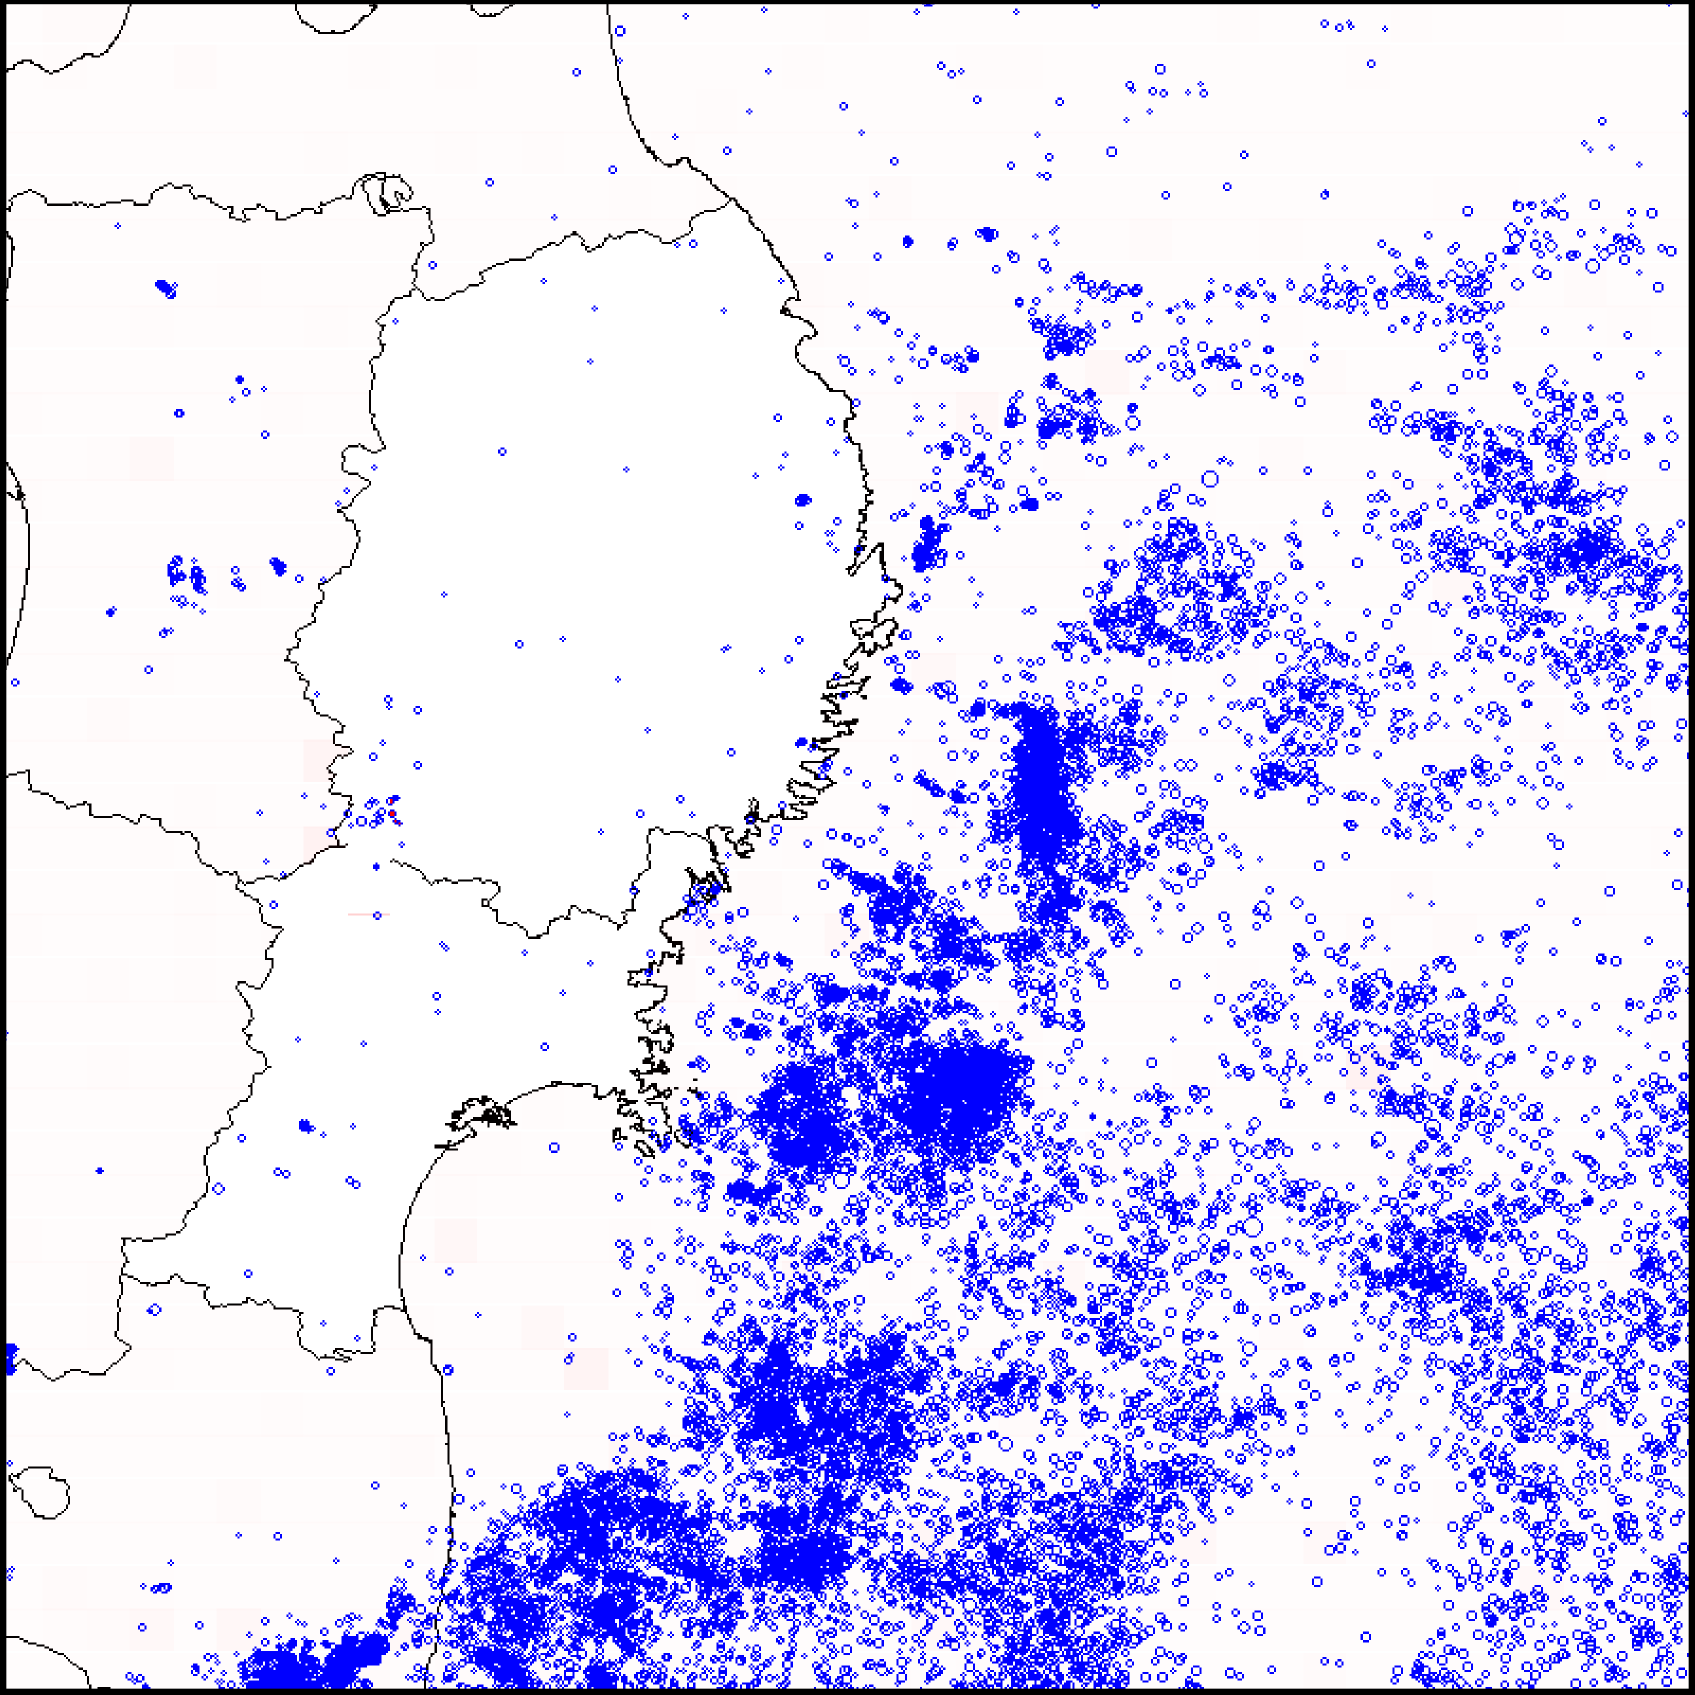
\includegraphics[width=0.4\textwidth]{img/tohokuoki.png}
  \end{center}
  \caption{Seismic Activity in Eastern Japan in 2011. Each circle
    represents one earthquake}
  \label{touhokuoki}
\end{figure}
%% TODO: Melhorar o caption desta figura, nao esta claro o que ela
%% representa.

Earthquakes pose a great risk for human society, in their potential
for large scale loss of life and destruction of infra-structure. In
the last decade, large earthquakes such as Sumatra (2004), Kashmir
(2005), Sichuan (2008) and Tohoku (2011, shown in
Figure~\ref{touhokuoki}) caused terrible amounts of casualties.

It is crucially important to understand the patterns and mechanisms
behind the occurrence of earthquakes. This knowledge may allow us to
create better seismic risk forecast models, indicating which regions
show a higher probability of earthquake occurrence at certain periods
in time. Such information can be put to good use for mitigating damage
through urban planning, civil engineering codes, emergency
preparedness, et cetera.

Earthquake ``prediction'' is a polemic subject. No research so far has
even come close to suggesting that individual large scale earthquakes
can be predicted with any sort of precision. On the other hand, it is
clear that at the very least earthquakes do cluster in time and
space. There is a lot of value behind the study of earthquake
mechanisms, with the goal of generating statistical models of
earthquake risk~\cite{Nature1999}.

Surprisingly enough, applications of Evolutionary Computation (EC) for
the problem of earthquake forecasting have been few and far
between. Given that EC has some times managed to find better solutions
than humans for hard problems~\cite{Koza2003}, we wonder if Artificial
Evolution might not be able to find new ideas that improve our
understanding of earthquakes and their processes.

With this in mind, the goal of this paper is to explore the
suitability of Evolutionary Computation to the problem of generating
earthquake forecast models. We aim to provide two main contributions:
\begin{enumerate}
\item Outline the earthquake forecast problem, which can be used as a
  foundation for other researchers who wish to contribute to this
  field.
\item Show that Evolutionary Computation is a promising methodology
  for the creation of earthquake forecast models, providing the
  motivation for further research in this direction. 
\end{enumerate}

It is important to note that our goal is not to generate an
``earthquake alarm system''. Rather, we use Evolutionary Algorithms to
find patterns that can be useful for further understanding the
mechanisms behind earthquake occurrence.

A common problem with applications of evolutionary algorithms is how
to compare different methods, developed by different groups with
different testing protocols, in a scientific fashion. We survey and
summarize the ``best practices'' for the studying and testing of
earthquake forecast models, as suggested by the \emph{Collaboratory
  for the Study of Earthquake Predictability} (CSEP), an international
partnership to promote rigorous study of the feasibility of earthquake
forecasting and predictability.

Based on this framework, we design and implement a simple Genetic
Algorithm for earthquake forecast modeling (\emph{GAModel}). We
compare forecasts generated by the GAModel with the Relative Intensity
algorithm (RI) and an information-less forecast. These systems are
applied on the earthquake catalog from the Japanese Meteorological
Agency (JMA), using event data from 2005 to 2012. The forecasts are
analyzed by their log-likelihood values compared to the actual data,
as suggested in the Regional Earthquake Likelihood Model (RELM), and
by the Area Skill Score (ASS) test.

The forecasts created by the GAModel were generally competitive in
relation to the RI algorithm, specially in scenarios with large amount
of inland seismic activity. We discuss some of the strong and weak
points identified from the experiment. The results overall show that
while there is vast room for improvement, Evolutionary Algorithm
approaches definitely have potential in this field.

%% I hate this kind of paragraph.
The paper is organized as follows: in Section 2 we detail the
earthquake forecast problem, and the CSEP framework. Section 3 reviews
applications of Evolutionary Computation in the context of seismology
research. In Section 4 we detail the proposed Genetic Algorithm system
for generating earthquake forecasts. In Section 5 we present the
results of the comparisons between this system and the RI
algorithm. In Section 6 we discuss the implications of the results and
conclude the paper.

%%%%%%%%%%%%%%%%%%%%%%%%%%%%%%%%%%%%%%%%%%%%%%%%%%%%%%%%%%%%%%%%%%%
\section{The Earthquake Forecasting Problem}
%% DONE, needs proofreading

In the field of seismology, there is a large number of model proposals
for earthquake forecasting. These proposals range from methods based
on geophysical principles to purely statistical algorithms.

In this context, the \emph{Collaboratory for the Study of Earthquake
  Predictability} (CSEP)\footnote{http://www.cseptesting.org} proposes
a methodology for rigorous scientific testing of these many different
models.

This testing happens mainly in the shape of distributed virtual
laboratories~\cite{Nanjo2011b}. Multiple research groups will submit
their forecast models, which will be compared against future
earthquake event data, using standardized testing protocols. The
testing suite used in these comparisons is made publicly available by
the CSEP, so that researchers can develop and test their models
beforehand.

In many application domains, the lack of an unified testing protocol
means that comparing methods developed by different research groups
can be a great burden. The CSEP framework allows us to objectively and
consistently compare our proposed algorithms with previous approaches.

\subsection{Earthquake Forecast Model}\label{CSEP_definition} 
%% DONE, needs proofreading

\begin{figure}
  \begin{center}
    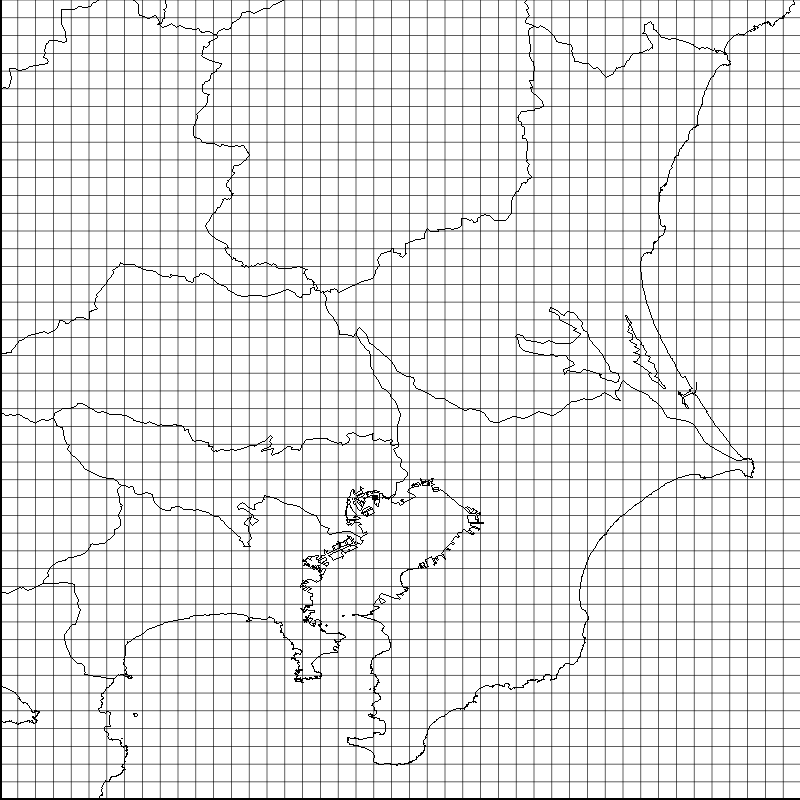
\includegraphics[width=0.45\textwidth]{img/kantomap.png}
  \end{center}
  \caption{Target area for the Kanto region and its bins}
  \label{fig:kantomap}
\end{figure}

In the CSEP framework, a forecast exists in reference to a
geographical region, a start date and an end date. The forecast will
estimate the number (and sometimes the magnitude) of earthquakes
that happens in this target region, during the target time interval.

A forecast is divided into bins. Each bin represents a non-overlapping
geographical interval within the target region, and sometimes also a
magnitude interval.

For example, in this paper we define the ``Kanto'' region as as the
area covered by latitude N34.8 to N36.3, and longitude E138.8 to
E140.3. This area is divided into 2025 bins (a grid of 45x45
squares). Each bin has an area of approximately $25km^2$
(Figure~\ref{fig:kantomap}).

For each bin in the forecast we define a number of expected
earthquakes. This number must be a positive integer. A good forecast
is one where the number of estimated earthquakes in each bin
corresponds to the actual number of earthquakes that occurs in that
bin during the target time interval.

\subsection{Comparison Testing}\label{CSEPTests}

The CSEP framework uses six different tests to compare earthquake
forecasts. These are divided into two groups: log-likelihood based
tests, and alarm based tests.

The first group is based on the analysis of the similarity between the
forecast and the actual earthquake catalog, following the Regional
Earthquake Likelihood Model (RELM)~\cite{Schorlemmer2007}. The log
likelihood of the forecast, given the actual data, is calculated using
a Poisson's probability distribution. From this data, three tests are
defined. The \emph{L-test} compares the difference between the
log-likelihood of the forecast against the actual data, and the
log-likelihood of the forecast against itself. The \emph{N-test} tests
whether the forecast is predicting too many or too few events in
total, and the \emph{R-test} provides an algorithm for the statistical
testing of multiple forecasts at once.

These tests require that all forecasts under comparison have the same
number and size of bins. Also, due to the way the log likelihood is
calculated, they pose a restriction on the forecast: if any one bin in
the forecast has zero earthquakes, while the corresponding bin in the
data has one or more events, the entire forecast is discarded.

Alarm based tests, on the other hand, use a threshold
analysis~\cite{Zechar2010}. For a given forecast a numerical threshold
is decided: all bins with forecast values above the threshold are
added to an alarm set. Earthquakes that fall in this alarm set are
counted as hits, while those falling outside the alarm set are counted
as misses. Alarm based tests rely on two values: a miss rate $v$, the
proportion of misses to the total number of earthquakes; and the
coverage rate $\tau$, the smallest alarm set necessary to achieve $v$.

Three alarm based tests are defined. The \emph{Molcham Diagram} draws
a path of $v$ and $\tau$ based on varying values of the threshold. The
\emph{Area Skill Score (ASS)} is defined as the area of the curve
under the Molcham diagram, and can be used to summarize the
information from the Molcham diagram as a single number. Finally, a
\emph{Receiver Operation Characteristic (ROC)} analysis can be done
from $v$ and $\tau$. Alarm based tests can compare forecasts with
different bin sizes, but they do not directly take into account the
total number of earthquakes on the forecast, or the data.

\section{Evolutionary Computation for Earthquake Risk Analysis}
%% DONE, needs proofreading

Reports of the application of Evolutionary Computation and related
methods for the generation of earthquake forecasts are rather sparse.
One such approach is described by Zhang and
Wang~\cite{Zhang2012}. They use Genetic Algorithms to fine tune an
Artificial Neural Network (ANN), and use this system to produce a
forecast. Unfortunately that paper did not provide enough information
to reproduce the proposed GA+ANN system or their results. Zhou and
Zu~\cite{Feiyan2014} also recently proposed a combination of ANN and
EC, but their system only forecasts the magnitude parameter of
earthquakes.

On the other hand, there are quite a few works using Evolutionary
Computation methods for the estimation of parameter values in
seismological models. These models are used to describe and understand
particular characteristics of earthquakes or earthquake activity.

For example, there are many examples of using Evolutionary Computation
to estimate the peak ground acceleration of seismically active
areas~\cite{Kermani2009,Cabalar2009,Kerh2010}. Ramos~\cite{Ramos2011}
used Genetic Algorithms to decide the location of sensing stations in
a seismically active area in Mexico. Nicknam et al.~\cite{Nicknam2010}
and Kennett and Sambridge~\cite{Kennett1992} used evolutionary
computation to determine the Fault Model parameters (such as epicenter
location, strike, dip, etc) of a given earthquake.

\section{A Forecast Model Using Genetic Algorithms}\label{implementation}
%% DONE, needs proofreading

To investigate the ability of Evolutionary Computation to generate
earthquake forecast models, we design and test a simple Genetic
Algorithm. We call this system the \emph{GAModel}.

An individual's genome in GAModel encodes a forecast model as defined
in the CSEP framework~(see Section~\ref{CSEP_definition}). The
population is trained on earthquake occurrence data for a fixed
training period, which is anterior to the target test period. After
the stopping criterion is reached, the best individual is taken as the
final forecast.

By encoding the entire forecast as the genome of one individual, we
identify two concerns that must be addressed by any EC-based
approach: First, as forecast models normally include a few thousand
bins, an individual's genome will be correspondingly
large. Evolutionary operators and parameters must be chosen to
guarantee convergence in a reasonable time frame.

Second, the design of the fitness function deserves a lot of
attention, to avoid the risk of over fitting the system to the
training data.

\subsection{Genome Representation}
%% DONE, needs proofreading

In GAModel, each individual represents an entire forecast model. The
genome is a real valued array $X$, where each element corresponds to
one bin in the desired model (the number of bins $n$ is defined by the
problem). Each element $x_i \in X$ takes a value from $[0,1)$. In the
  initial population, these values are sampled from a uniform
  distribution.

In the CSEP framework, a model is defined as a set of integer valued
expectations, corresponding to the number of earthquakes for each
bin. To convert from the real valued chromosome to a integer forecast,
we use a modification of the Poisson deviates extraction algorithm
from~\cite{NumericalRecipes}~(Chapter 7.3.12).

\begin{algorithm}
  \caption{Obtain a Poisson deviate from a $[0,1)$ value}
  \label{InversePoisson}
  \begin{algorithmic}
    \STATE Parameters $0 \leq x < 1, \mu \geq 0$
    \STATE $L \gets \exp{(-\mu)}, k \gets 0, prob \gets 1$
    \REPEAT 
    \STATE $\text{increment }k$
    \STATE $prob \gets prob*x$
    \UNTIL{$prob > L$}
    \RETURN $k$
  \end{algorithmic}
\end{algorithm}

In Algorithm~\ref{InversePoisson}, $x$ is the real value taken from
the chromosome, and $\mu$ is the average number of earthquakes
observed across the entire training data. Note that in the original
algorithm, $k-1$ is returned. Because the log likelihood calculation
used for model comparison discards forecasts that estimate zero events
in bins where earthquakes are observed, we modify the original
algorithm to make sure all bins estimate at least one event.

\subsection{Fitness Function}

Usually, the main challenge when applying an Evolutionary Computation
method to any new application domain is the definition of an
appropriate fitness function. Accordingly, a large part of our effort
was to define a good fitness function for GAModel.

We describe two candidate fitness functions. The first one is a direct
application of the log likelihood definition for earthquake
forecast. Because this fitness function resulted in an excessive
amount of over fitting, we describe a second fitness function that
breaks the training data set into smaller data sets in order to avoid
this problem.

\subsubsection{Simple Log Likelihood Fitness Function} 

This fitness function uses the log-likelihood between the forecast
generated by an individual and the observed earthquakes in the
training data, as described by Schorlemmer et
al.~\cite{Schorlemmer2007}. In simple terms, the log likelihood is a
measure of how close a forecast is to a given data set.

Let $\Lambda = \{\lambda_1, \lambda_2, \dots, \lambda_n | \lambda_i
\in \mathbb{N}\}$ be a forecast with $n$ bins. In this definition,
$\lambda_i$ is the number of earthquakes that is forecast to happen in
bin $i$. To derive $\Lambda_X$ from an individual $X = \{x_1, x_2,
\dots, x_n | 0 \leq x_i < 1\}$, we calculate each $\lambda_i$ from
$x_i$ using Algorithm~\ref{InversePoisson}.

Now, let $\Omega = \{\omega_1, \omega_2, \dots, \omega_n | \omega_i
\in \mathbb{N}\}$ be the observed numbers of earthquakes for each bin
$i$ in the training data. The log likelihood between an individual's
forecast $\Lambda_X$ and the observed data $\Omega$ is calculated as:
\begin{equation}
  L(\Lambda_X|\Omega) = \sum_{i=0}^n {-\lambda_i +
    \omega_i*\ln(\lambda_i)-ln(\omega_i!)}
\end{equation}
There are two special cases that arise when any $\lambda_i = 0$. If
$\lambda_i = 0$ and $\omega_i = 0$, then the value of the sum for that
element is $1$. If $\omega_i > 0$, then $L(\Lambda_X|\Omega) =
-\infty$ and the forecast must be discarded. For more details on
this, see~\cite{Schorlemmer2007}.

In the Simple Log Likelihood fitness function, the value of
$L(\Lambda_X|\Omega)$ is taken directly as the fitness value of the
individual.

Early testing with the Simple Log Likelihood function showed that
GAModel had a very strong tendency to over fit to the training
data. This is natural, since there are differences between the
seismicity of a larger period and a shorter one. To solve this
problem, we used the fitness function shown in the next section.

\subsubsection{Time-slice Log Likelihood Fitness Function}

In the time-slice log likelihood fitness function we break up the
training data set into smaller slices. These slices are based on the
chronology of the earthquakes contained in the training catalog. The
duration of each slice is the same as the duration of the target
interval (the test data).

Let's consider an example: the target period for the forecast is one
year, from 1/1/2014 to 1/1/2015, and the training data is taken from
the 10 year period between 1/1/2004 and 1/1/2014. To apply the
time-slice log likelihood fitness function, we divide the training
data into ten 1-year slices, from 2004 to 2005, 2005 to 2006, and so
on.

When an individual $X$ is evaluated, we calculate the log likelihood
of its forecast $\Lambda_X$ against each of the time slices
($\Omega_{2004}, \Omega_{2005}, \dots, \Omega_{2013}$). We use the
lowest log likelihood value from among all the slices as the fitness
of $X$.

The idea behind this fitness function is that the catalog data
available for training will normally span a period of time much longer
than the desired forecast. By breaking the training data into smaller
periods, we are trying to make the evolutionary algorithm learn any
time-repeating pattern that might exist in the data. We choose the
smallest log likelihood from the time slices in order to make sure
that the evolution process favors solutions that try to solve all
slices equally.

\subsection{Evolutionary Operators and Parameters}

GAModel uses a regular generational genetic algorithm. For selection,
we use Elitism and Tournament selection.

We use a simple Uniform Crossover for the crossover operator. If a
gene's value falls outside the $[0,1)$ boundary, it is truncated to
  these limits. For the mutation operator, we sample entirely new
  values from $[0,1)$ for each mutated chromosome.

\begin{table}[!ht]
  \caption{Parameters used in GAModel}
  \label{GAParameters}
  \begin{center}
  \begin{tabular}{|l|r|}
    \hline
    Population Size & 500\\
    Generation Number & 100\\
    Elite Size & 1\\
    Tournament Size & 50\\
    Crossover Chance & 0.9\\
    Mutation Chance (individual) & 0.8\\
    Mutation Chance (chromosome) & (genome size)$^{-1}$\\
    \hline    
  \end{tabular}
  \end{center}
\end{table}

The parameters used for the evolutionary computation are described in
Table~\ref{GAParameters}. Because our focus is to show the viability
of Evolutionary Algorithms for this application problem, we are not
yet particularly concerned with the convergence speed of the
system. Accordingly, not a lot of effort was spent fine tuning these
parameter values. These values were chosen instead by trial and error
on a data region not used in the experiments of Section~\ref{data},
until an acceptable convergence time was found.

\section{Experiments}

To analyze the performance of the forecasts generated by the GAModel,
execute a simulation experiment. In this simulation, the GAModel
evolves using a training data set, and the resulting forecast is
analyzed against a test data set. These results are compared against
two other forecasts: an ``unskilled'' forecast, which randomly guesses
the forecast~(Figure~\ref{randomforecast}), and a forecast generated by the
Relative Intensity (RI) algorithm, regarded as a natural reference for
comparative tests with any type of forecast models~\cite{Nanjo2011}.

\subsection{Experimental Data}\label{data}

The data used in these experiments comes from the Japan Meteorological
Agency's (JMA) catalog. The catalog lists earthquakes recorded by the
sensing station network in Japan. For each earthquake, the following
values are given: time of occurrence, magnitude, latitude and
longitude and depth of the hypocenter.

We consider events with magnitude above 2.5 and depth less than 100km,
recorded in the period from 2000 to 2013. This accounts for more than
220.000 earthquakes in the Japanese archipelago.

To achieve a better understanding of the forecasting power of GA
models, we define four areas to focus as scenarios in our
experiment. Figure~\ref{areamap} shows where these four areas are
located. Three of these areas (Kanto, Touhoku and Kansai), contain
mainly inland earthquakes, which are considered to follow more stable
patterns. The fourth area (East Japan) includes also many off-shore
earthquakes.  To make it easier to compare the results for each area,
we choose the bin size so that the total number of bins is within the
same order of magnitude in all areas.

\begin{enumerate}
  \item {\bf Kanto:} Kanto is the area at and nearby Tokyo. There is a
    large amount of seismic activity in the target period. In this
    study, we define this region as starting at N34.8,W138.8, with
    2025 bins arranged in a 45x45 grid. Each bin corresponds to a
    5km$^2$ square.
  \item {\bf Kansai:} The Kansai area includes Kyoto, Osaka, Kobe and
    nearby cities. This area shows a relatively lower amount of
    seismic activity in the period considered. We define this region
    as starting at N34,W134.5, with 1600 bins arranged in a 40x40
    grid. Each bin corresponds to a 5km$^2$ square.
  \item {\bf Touhoku:} The Touhoku region is defined as the northern
    provinces of the main island. It shows some clusters of seismic
    activity during the period studied. We define this region as
    starting at N37.8,W139.8, with 800 bins arranged in a 40x20
    grid. Each bin corresponds to a 10km$^2$ square.
  \item {\bf East Japan:} This area corresponds to Japan's
    north-eastern coast. It includes both inland and off-shore events,
    which makes it more difficult to forecast. It also includes the
    location of the M9 earthquake of 2011. We define this region as
    starting at N37,W140, with 1600 bins arranged in a 40x40
    grid. Each bin corresponds to a 10km$^2$ square.
\end{enumerate}

\begin{figure}
  \begin{center}
  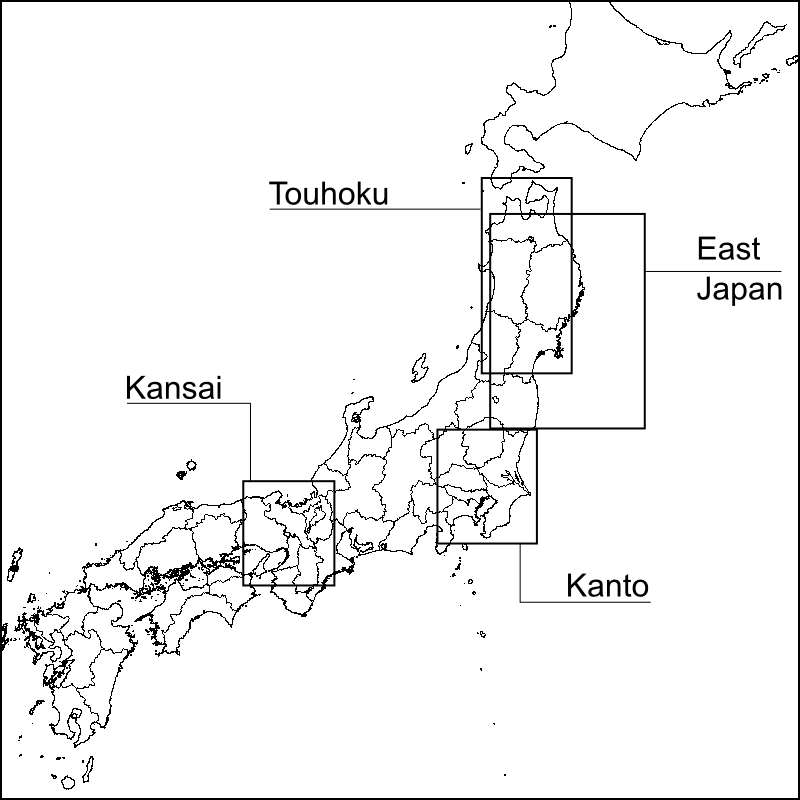
\includegraphics[width=0.40\textwidth]{img/alljapan.png}
  \end{center}
  \caption{The relative locations of the four areas used in our
    experiments}
  \label{areamap}
\end{figure}

\subsection{Experimental Design} %% DONE

To compare the performance of the different forecast models, we
execute a simulation experiment on 32 scenarios. A scenario is defined
by a target region and a target time interval. The region is selected
from the four regions described in the previous section. The time
interval is a one year interval, lasting from Jan/01 to Dec/31. We
consider 8 periods (from 2005 to 2012). In each period, we use 5 years
of prior data (2000 to 2011) to train the RI and GAM algorithms.

For each scenario, we generate forecasts for the random model, the GAM
model (using the second fitness function described in this paper) and
the RI model. The random forecast is generated by selecting a random
uniform value between 0 and 1 for each bin, and transforming this
value into an integer using Algorithm~\ref{InversePoisson}. The RI
forecast is generated according to Section~\ref{RI}.

Both the GAModel and the RI algorithm require a training data set. For
each scenario, we use earthquake data from the 5 year period
immediately prior to the testing period. In order to test the
statistical significance of our results, we run the GAModel 20 times,
and obtain 20 forecasts. All GAModel results, unless noted otherwise,
are the mean of these 20 runs. Because the RI algorithm is not
stochastic, the result of a single run is reported.

The results are compared in mainly two ways. We report the
log-likelihood values for the three methods. The log likelihood
indicates how close the forecast is to the test data, in terms of
location and quantity of earthquakes. We also report the Area Skill
Score (ASS) for the three methods. The ASS is the area covered by the
``Alarm rate x Miss rate'' curve of the forecast~(see
Section~\ref{CSEPTests} for details). In both cases, a higher value
indicates a more skilled model.


%% Image: Random
\begin{figure}
  \begin{center}
    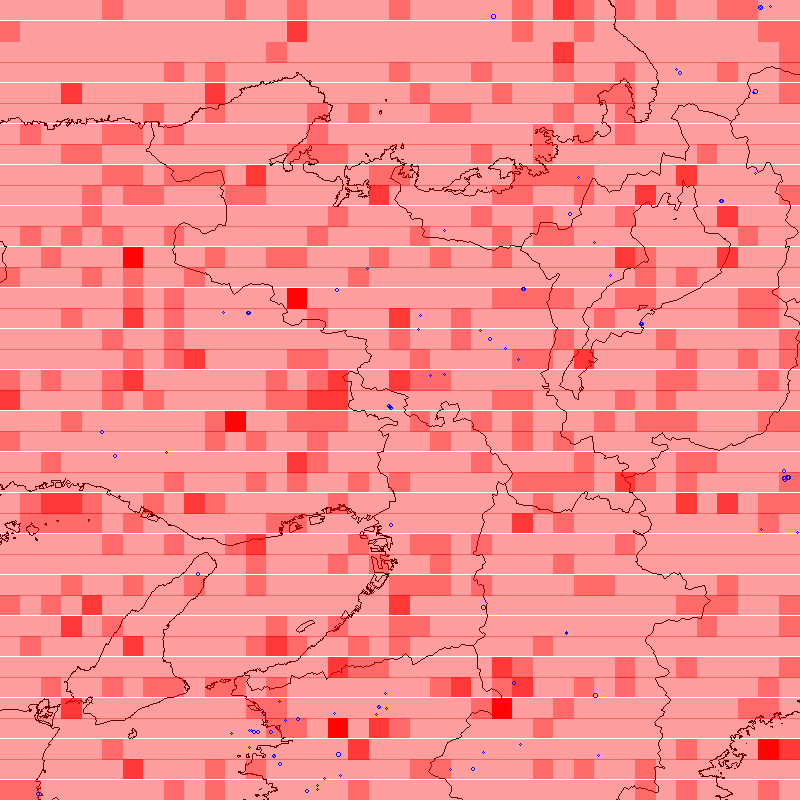
\includegraphics[width=0.4\textwidth]{img/kansai07_random.png}
  \end{center}
  \caption{A random forecast (Kansai Region, 2007)}
  \label{randomforecast}
\end{figure}

\subsection{The Relative Intensity Algorithm}\label{RI}

The Relative Intensity (RI) algorithm is a commonly used benchmark for
earthquake forecasting models. In this experiment, we use it as
goalpost to assess the suitability of evolutionary computation for
earthquake forecasting.

The working assumption behind the RI is that larger earthquakes are
more likely to occur at locations of high seismicity in the
past. Accordingly, the RI algorithm will estimate the number of
earthquakes in a bin based on the number of earthquakes observed in
the past for that bin. This estimate will be ``smoothed'' by an
attenuation factor $s$ that takes into account the seismicity of
neighboring bins.

We use the implementation described by Nanjo
in~\cite{Nanjo2011}. Please refer to that paper for implementation
details. The parameters used for the RI algorithm in these experiments
are: $b = 0.8$ and $s = 50km$. These values were selected by taking
the suggested range of values recommended in~\cite{Nanjo2011}, and
finding the best values in this range on the same data set used to
tune the parameters of the Genetic Algorithm.

\begin{table*}[t!]
  \caption{Results from the simulation experiments. The parenthesis
    after the GA values are the standard deviation (average of 20
    runs). The two ``p-value'' columns report the significance of the
    mean-test for the alternate hypothesis ``The GA average is higher
    than the RI result''. For the sake of legibility, p-values under
    $0.01$ are reported as $0.01$}
  \label{bigtable}
  \begin{center}
  \begin{tabular}{|ll||c|c|c|c||c|c|c|c|}
    \hline
    \multicolumn{2}{|c|}{Scenario} & \multicolumn{4}{|c|}{Log Likelihood} & \multicolumn{4}{|c|}{Area Skill Score}\\
     & & Random & RI & GA & p-value & Random & RI & GA & p-value\\
    \hline
    Kanto & 2005 &-3716.86 & -2263.4&-2253.2 (16.5) & 0.01 & 0.38 & 0.24 & 0.24 (0.04) & 0.78\\
    & 2006 &-3884.85 & -2252.28     &-2234.72 (14) & 0.01 & 0.36 & 0.10 & 0.18 (0.01) & 0.01 \\
    & 2007 &-3838.9 & -2113.84      &-2108.95 (11.1) & 0.03 & 0.36 & 0.15 & 0.19 (0.02) &  0.01 \\
    & 2008 & -3914.54&-2110.79      &-2096.75 (11.8) & 0.01 & 0.39 & 0.16 & 0.22 (0.03) & 0.01 \\
    & 2009 &-4211.28 &-2487.88      &-2482.88 (10.3) & 0.02 & 0.36 & 0.09 & 0.14 (0.01) & 0.01 \\
    & 2010 & -4010.47&-2132.11      &-2099.13 (16.3) & 0.01 & 0.39 & 0.14 & 0.28 (0.03) & 0.01 \\
    & 2011 &-17657.43 &-20083.09    &-19983.73 (144.4) & 0.01 & 0.35 & 0.07 & 0.08 (0.02) & 0.14\\
    & 2012 & -10863.99&-3225.39     &-4435.34 (248) & 1.00 & 0.48 & 0.80 & 0.77 (0.01) & 1.00 \\
    \hline
    Kansai & 2005 &-2219.06 &-1605 &-1631.96 (26) & 0.99 & 0.24 & 0 & 0.07 (0.02) & 0.01 \\
    & 2006 & -2172.29&-1606 &-1631.19 (23.9) & 0.99 & 0.23 & 0 & 0.05 (0.01) & 0.01 \\
    & 2007 &-2024.77 &-1615 &-1617.01 (2.3) & 0.99 & 0.22 & 0 & 0.03 (0.01) & 0.01 \\
    & 2008 &-2038.16 &-1608 &-1610.41 (1.54) & 1.00 & 0.22 & 0 & 0.01 (0.01) & 0.01 \\
    & 2009 &-2054.23 &-1618 &-1619.51 (2.58) & 0.99 & 0.21 & 0 & 0.02 (0.01) & 0.01 \\
    & 2010 & -2054.63&-1613 &-1611.00 (2.27) & 0.01 & 0.27 & 0 & 0.07 (0.02) & 0.01 \\
    & 2011 &-2059.89 &-1625 &-1625.12 (2.46) & 0.58 & 0.26 & 0 & 0.05 (0.03) & 0.01 \\
    & 2012 &-2080.35 &-1601 &-1603.59 (2.92) & 0.99 & 0.22 & 0 & 0.04 (0.02) & 0.01 \\
    \hline
    Touhoku & 2005 &-2552.61 &-1067.38 &-984.23 (84) & 0.01 & 0.58 & 0.58 & 0.62 (0.01) & 0.01 \\
    & 2006 &-2613.1 &-1044.72 &-1073.03 (154) & 0.78 & 0.52 & 0.50 & 0.42 (0.03) & 1.00\\
    & 2007 & -2666.11&-1049.82 &-999.64 (83.6) & 0.01 & 0.51 & 0.51 & 0.41 (0.01) & 1.00\\
    & 2008 & -5124.54&-5007.49 &-4704.15 (131) & 0.01 & 0.36 & 0.05 & 0.18 & 0.01\\
    & 2009 & -2737.47&-1049.22 &-936.63 (60) & 0.01 & 0.54 & 0.67 & 0.70 (0.01) & 0.01\\
    & 2010 & -2714.68&-1045.03 &-1077.95 (136) & 0.85 & 0.53 & 0.66 & 0.57 & 1.00\\
    & 2011 & -3435.67&-2753.95 &-2963.31 (88) & 1.00 & 0.40 & 0.21 & 0.10 (0.01) & 1.00\\
    & 2012 &-3623.22 &-1326.52 &-1186.1 (45.3) & 0.01 & 0.47 & 0.62 & 0.70 (0.05) & 0.01\\
    \hline
    East Japan & 2005 & -2666.11  &-1049.82 &-868.87 (20) & 0.01 & 0.47 & 0.35 & 0.30 (0.02) & 1.00 \\
    & 2006 & -6596.76 & -2130.69  &-2303.78 (98) & 1.00 & 0.46 & 0.42 & 0.35 (0.01) & 1.00 \\
    & 2007 & -6714.36 & -1997.78  &-2065.4 (85) & 0.99 & 0.43 & 0.51 & 0.34 (0.02) & 1.00 \\
    & 2008 &-8784.64  & -6087.88  &-6097.63 (264) & 0.56 & 0.46 & 0.23 & 0.20 (0.03) & 1.00 \\
    & 2009 & -6435.07 & -2052.35  &-1964.72 (106) & 0.01 & 0.47 & 0.49 & 0.48 (0.02) & 0.99\\
    & 2010 &-6560.97  & -2572.97  &-2541.33 (121) & 0.12 & 0.46 & 0.41 & 0.31 (0.01) & 1.00 \\
    & 2011 & -31447.79& -47704.35 &-51485.77 (536) & 1.00 & 0.44 & 0.40 & 0.18 (0.01) & 1.00 \\
    & 2012 & -19068.86& -5177.55  &-6657.52 (478) & 1.00 & 0.50 & 0.77 & 0.71 (0.01) & 1.00 \\
    \hline
  \end{tabular}
  \end{center}
\end{table*}

%% Images: Comparisons
\begin{figure*}[P]
  \begin{center}
    \subfloat[Touhoku 2009, RI forecast]{
      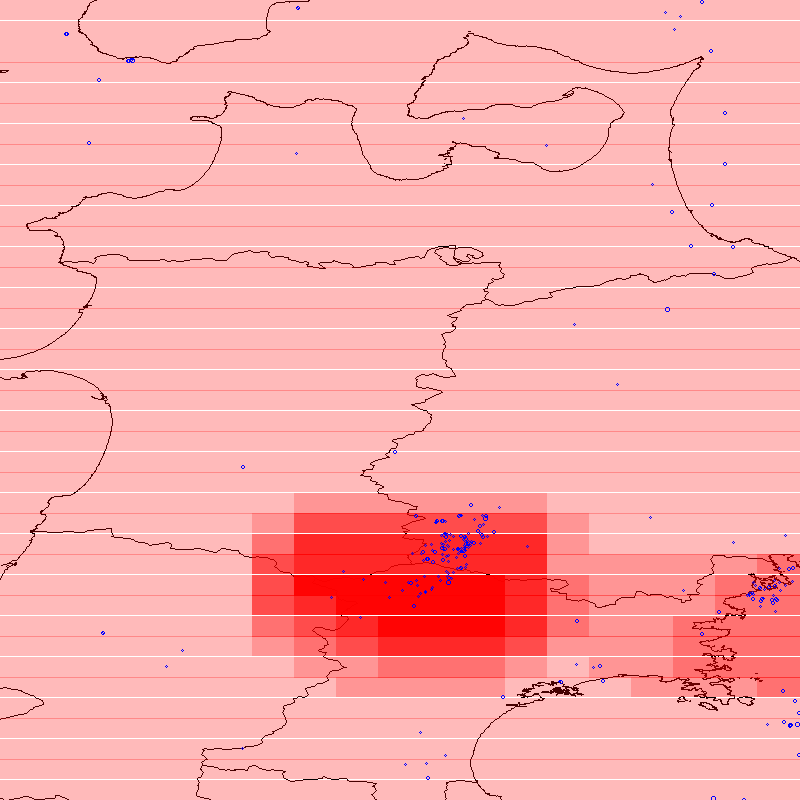
\includegraphics[width=0.38\textwidth]{img/touhoku09_RI.png}
      \label{fig:tohoku09ri}
    }
    \subfloat[Touhoku 2009, GA forecast]{
      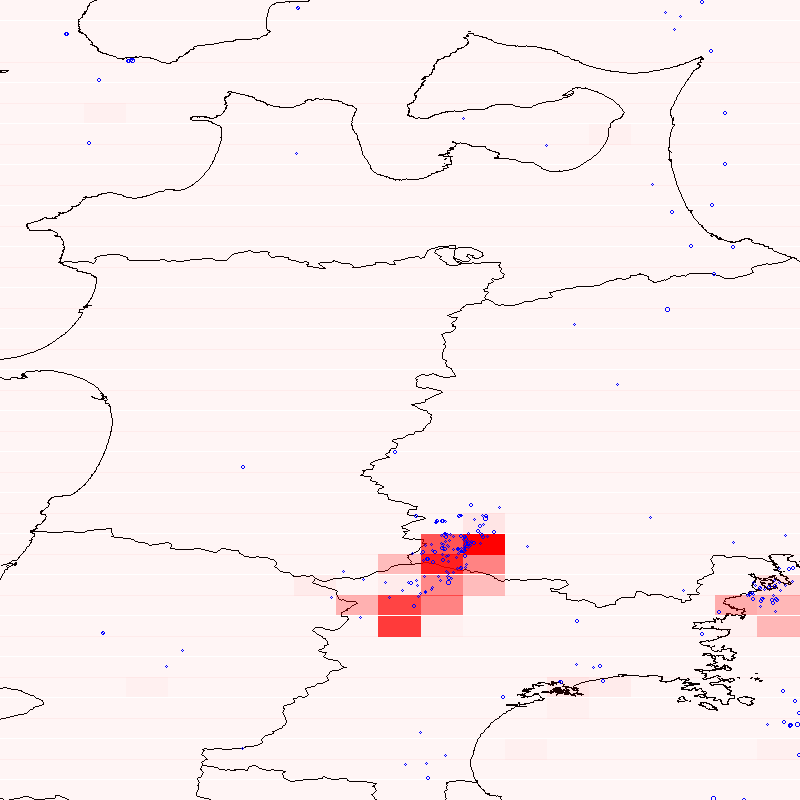
\includegraphics[width=0.38\textwidth]{img/touhoku09_ga.png}
      \label{fig:tohoku09ga}
    }
    
    \subfloat[Kanto 2010, RI forecast]{
      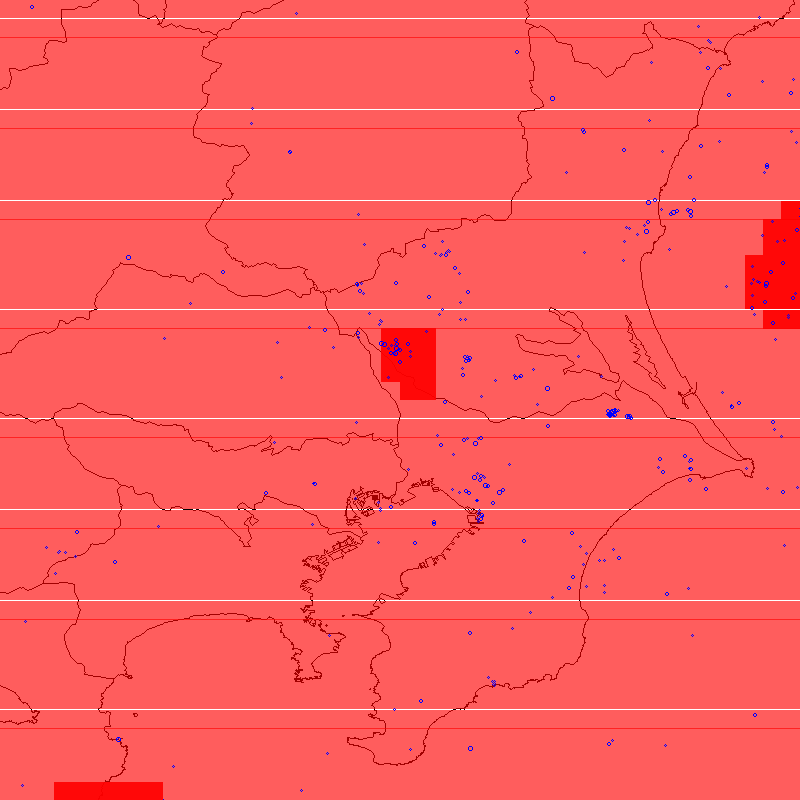
\includegraphics[width=0.38\textwidth]{img/kanto10_RI.png}
      \label{fig:kanto10ri}
    }
    \subfloat[Kanto 2010, GA forecast]{
      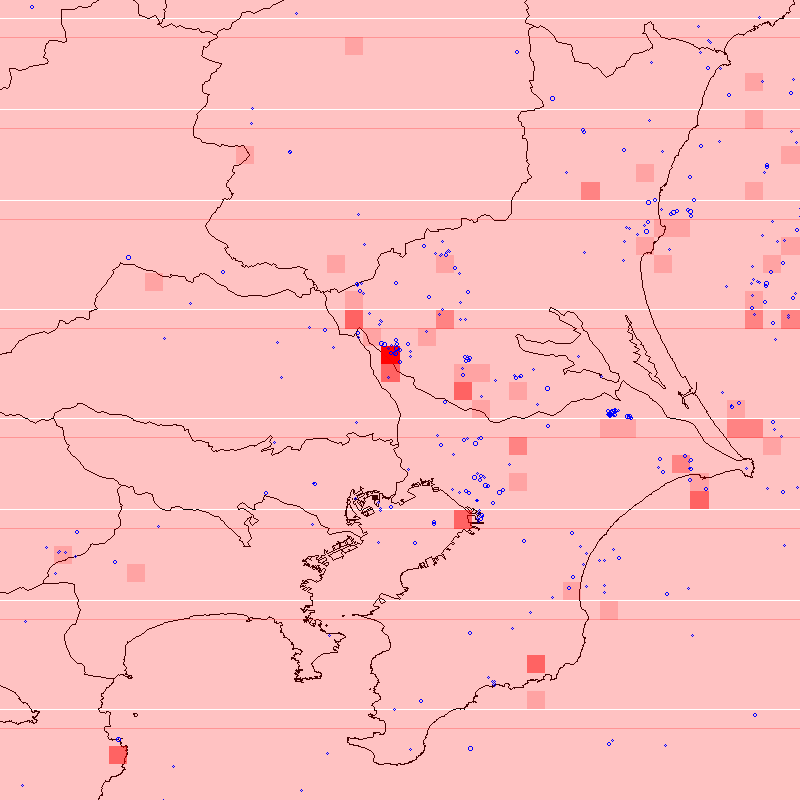
\includegraphics[width=0.38\textwidth]{img/kanto10_ga.png}
      \label{fig:kanto10ga}
    }

    \subfloat[Kanto 2012, RI forecast]{
      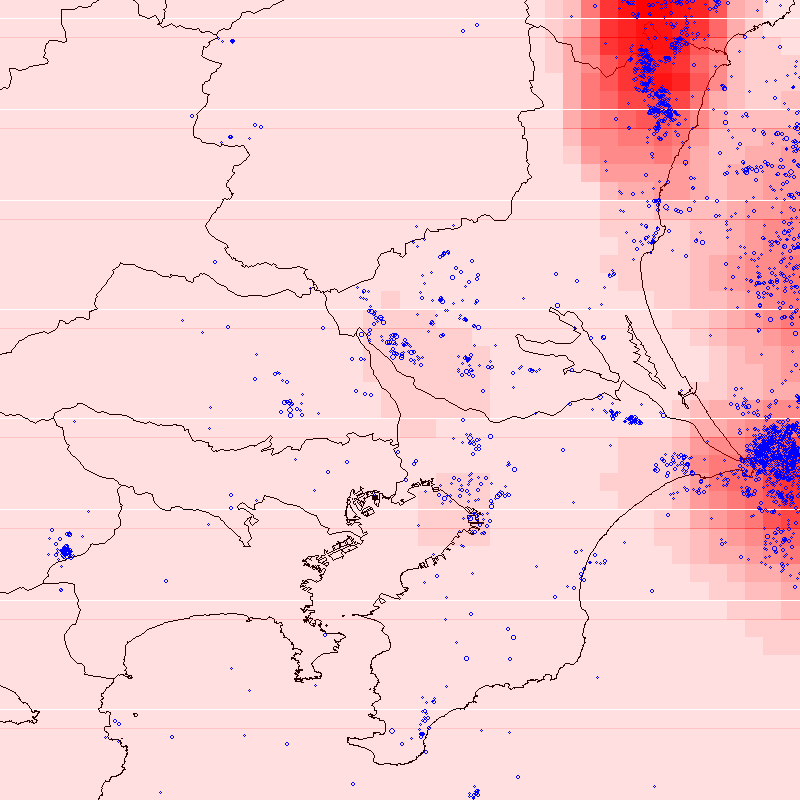
\includegraphics[width=0.38\textwidth]{img/kanto12_RI.png}
      \label{fig:kanto12ri}
    }
    \subfloat[Kanto 2012, GA forecast]{
      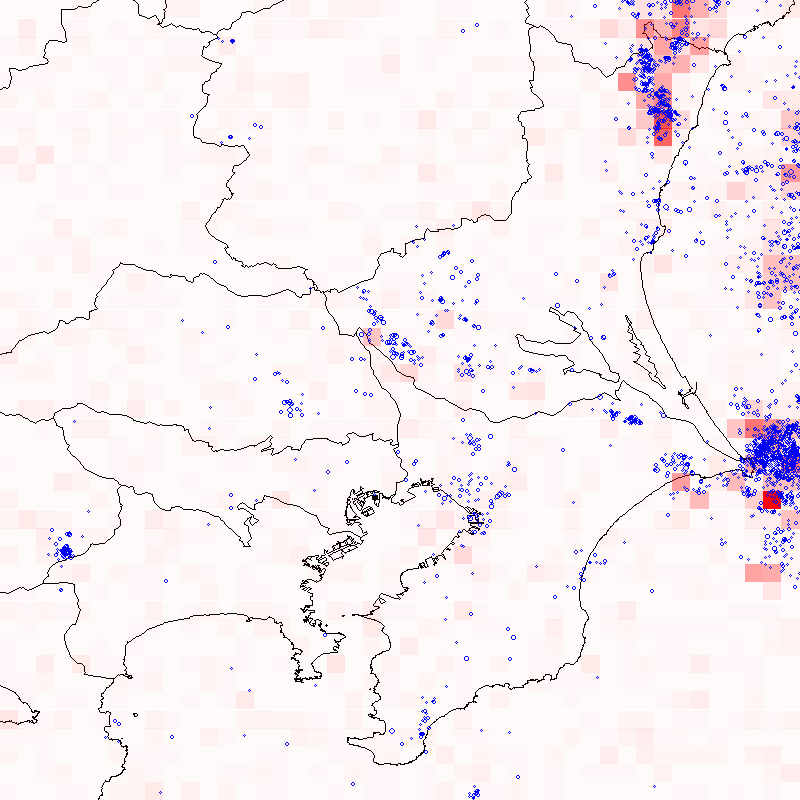
\includegraphics[width=0.38\textwidth]{img/kanto12_ga.png}
      \label{fig:kanto12ga}
    }
    
  \end{center}
  \caption{Some forecast images for the RI algorithm and the
    GAModel. Red squares indicate the intensity of the forecast. Blue
    circles indicate actual earthquakes in the test data. Note that
    the intensity of the red color indicates relative values in the
    forecast. In other words, uniform forecasts will tend to appear as
    a darker red color than forecasts with a bigger range of values.}
  \label{fig:results}
\end{figure*}


\subsection{Comparison of Forecast Models}

The results of the simulation experiments are summarized in
Table~\ref{bigtable}. In this table, \emph{Random} refers to the
Random forecast, \emph{RI} to the Relative Intensity algorithm, and
\emph{GA} to the GAModel. 

The GA column reports the average for 20 runs, and the standard
deviation is reported in parenthesis. The \emph{p-value} column
indicates the result of a one-sided T-test where the alternate
hypothesis is ``The GA average is greater than the RI result''.

Looking at the table, we observe that the GAModel has generally
outperformed the RI on the ``Kanto'' area. Figures~\ref{fig:kanto10ri}
and~\ref{fig:kanto10ga} illustrate the reason: Generally, GAModel is
able to detect smaller earthquake clusters inland, while RI smooths them
out. 

Even then, both models miss some clusters in this area, as indicated
by their ASS value being under the value of the random model. The ASS
value is useful to estimate how much a forecast is suffering from over
fitting - a low value indicates that a larger alarm area is necessary
to reduce the miss rate of the forecast.

The ``Touhoku'' area shows a similar situation as the ``Kanto''
area. In Figures~\ref{fig:tohoku09ri} and~\ref{fig:tohoku09ga} we can
see that GAModel is able to identify the two earthquake clusters more
precisely, while the RI algorithm casts a wide net which reduces the
forecast accuracy. The ASS score for this area is higher. This is
because both methods are able to learn the two ``hot spots'' for
seismic activity, unlike the Kanto area where some clusters would
appear in different locations along the years.

Conversely, in the ``East Japan'' area, the RI algorithm performed
better than the GAModel. The reason seems to be that off-shore
seismicity, which is spread over a larger area than inland events, is
better captured by the wide smoothing step of the RI algorithm.

In all three cases, we can see that the results changed wildly in the
aftermath of the 2011 M9 earthquake. That earthquake caused a sudden
large spike of seismic activity in all
areas~(Figure~\ref{touhokuoki}), including many areas that never
showed any seismic activity in the training period. In the following
scenario (2012), both methods try to use this new data to reform their
forecasts. Again, GAModel performs better in the ``Touhoku/2012''
scenario, where most earthquakes are inland. The RI method performs
better in the ``Kanto/2012'' scenario, where most of the new
seismicity occurs off-shore~(Figures~\ref{fig:kanto12ri}
and~\ref{fig:kanto12ga}).

The ``Kansai'' scenarios turned out to be a special situation for both
algorithms. The seismic activity for the period was too sparse. Since
both the RI and GAModel depend on the analysis of recent earthquakes,
neither algorithm could produce a reliable forecast. In the case of
the RI, the forecast produced was largely a uniform forecast, where
all bins had equal or very close expectation values. In the case of
GAModel, A few bins where earthquakes had happened in the training
data were marked with higher forecasts, but no consistent activity
clusters were identified. The log likelihood or ASS scores for these
scenarios can't really be used to compare the two methods.

\section{Conclusion}

Our goal in this work was to open the discussion about the feasibility
of Evolutionary Computation approaches for the important problem of
generating earthquake forecast models. The mechanisms of earthquake
generation are still not fully understood, which motivates us to use
self-adaptive methods such as Genetic Algorithms.

To illustrate our proposal, we designed GAModel, a traditional GA with
an specific fitness function that generates an earthquake forecast
based on recent seismic history. We performed simulation experiments,
and compared the results with the RI method, which is accepted in the
seismology community as a natural benchmark.

Our results show that the GAModel is competitive with the RI
algorithm, outperforming it in scenarios with a predominance of
in-land earthquakes, and being outperformed when there is a large
number of off-shore earthquakes. In this sense, we feel that the
answer to the question posed by the title of the paper should be
``Yes, it is promising to use EC to generate earthquake forecasts''.

That said, we have also identified many places where an Evolutionary
forecast generator could be improved. Although the time-slice fitness
function was designed to reduce over fitting, we still see that GAModel
generates ``sharp'' forecasts that are probably the result of some
degree of over fitting.

In this paper, we have decided to focus on the introduction of this
new problem domain to the evolutionary computation
community. Therefore, we limited ourselves to the traditional
GA. However, we visualize many possible research directions based on
the shortcomings demonstrated in the current research.

One way to mitigate the sharpness noticed in the results is by making
the algorithm aware of data locality. Based on the smoothing pattern
in the RI algorithm, we plan to develop a self-adaptive way to smooth
the results in the GAM. Also, because in the REML each bin is
ultimately evaluated independently of the neighboring bins, it is
feasible to imagine that separate areas in a forecast model could be
generated by using different parameters, or different algorithm
variations altogether.

Finally, we currently only uses historical data to build a
forecast. We are very interested in finding ways to add domain
knowledge into the system, such as the location of known faults, in
order to improve the forecast ability.

\section{Acknowledgments}

We thank the Japan Meteorological Agency for providing the earthquake
catalog used in this study.

\bibliographystyle{apalike}
{\small \bibliography{earthquake}}

\end{document}
